\chapter{Laser interferometers for gravitational-wave detection}

\section{Signal versus noise}
The factors that must be considered in the design of any detector can
be grouped into two categories: signal and noise. The ability to make
a claim of detection is largely dependent on the magnitude of the
signal to noise ratio (SNR). An SNR of 8 is desired for detection
confidence in LIGO. For laser interferometers, the strength of the GW
signal is proportional to the length of the arms and the amount of
power in the arms. (See Eq. \ref{}.) The change in the distance
between the mirrors, $\Delta L$, is bigger for a given strain the
longer the arms. And with more circulating power, the greater the
amount of power that will show up at the AS port for a given
displacement from the dark fringe. Therefore, the two fundamental ways
to make a GW produce a bigger signal in an interferometer are: 1) make
the arms longer, and 2) increase the circulating power.

No matter how large a signal one might have, it won't be found
confidently, or at all, if there is too much noise. The noise itself
is best grouped into categories of displacement noise and sensing
noise, which affect the length of the arms and the measurement of the
signal, respectively. Interferometers for GW detection are plagued
primarily by displacement noise below 70~Hz and sensing noise above
200~Hz.

In the next sections I will describe briefly the specific types of
displacement and sensing noises affecting the sensitivity of laser
interferometers. A summary of the noise budget is shown in
Fig. \ref{}. 


\subsection{Displacement noise} 
ground motion, thermal noise

seismic noise physically displaces the mirrors, resulting in changes in the length
of the arm. 

\subsection{Sensing noise}
stray light, shot noise

Shot noise is a quantum mechanical effect of the detection
of photons which creates uncertainty in the phase of the light, and
therefore the power, at the AS port.


\section{Power-recycled Fabry-Perot Michelson}
The typical detector configuration is a power-recycled Fabry-Perot
Michelson laser interferometer featuring suspended test masses in
vacuum as depicted in Figure \ref{fig:IFOschematic}. A diode-pumped,
power amplified, and intensity and frequency stabilized Nd:YAG laser
emits light at 1064~nm. The laser is directed to a Michelson
interferometer whose two arm lengths are set to maintain destructive
interference of the recombined light at the anti-symmetric (AS)
port. An appropriately polarized gravitational wave will
differentially change the arm lengths, producing signal at the AS port
proportional to the GW strain and the input power. The Fabry-Perot
cavities in the Michelson arms and a power recycling mirror (RM) at
the symmetric port are two modifications to the Michelson
interferometer that increase the laser power in the arms and therefore
improve the detector's sensitivity to GWs.

\begin{figure}
\begin{centering}
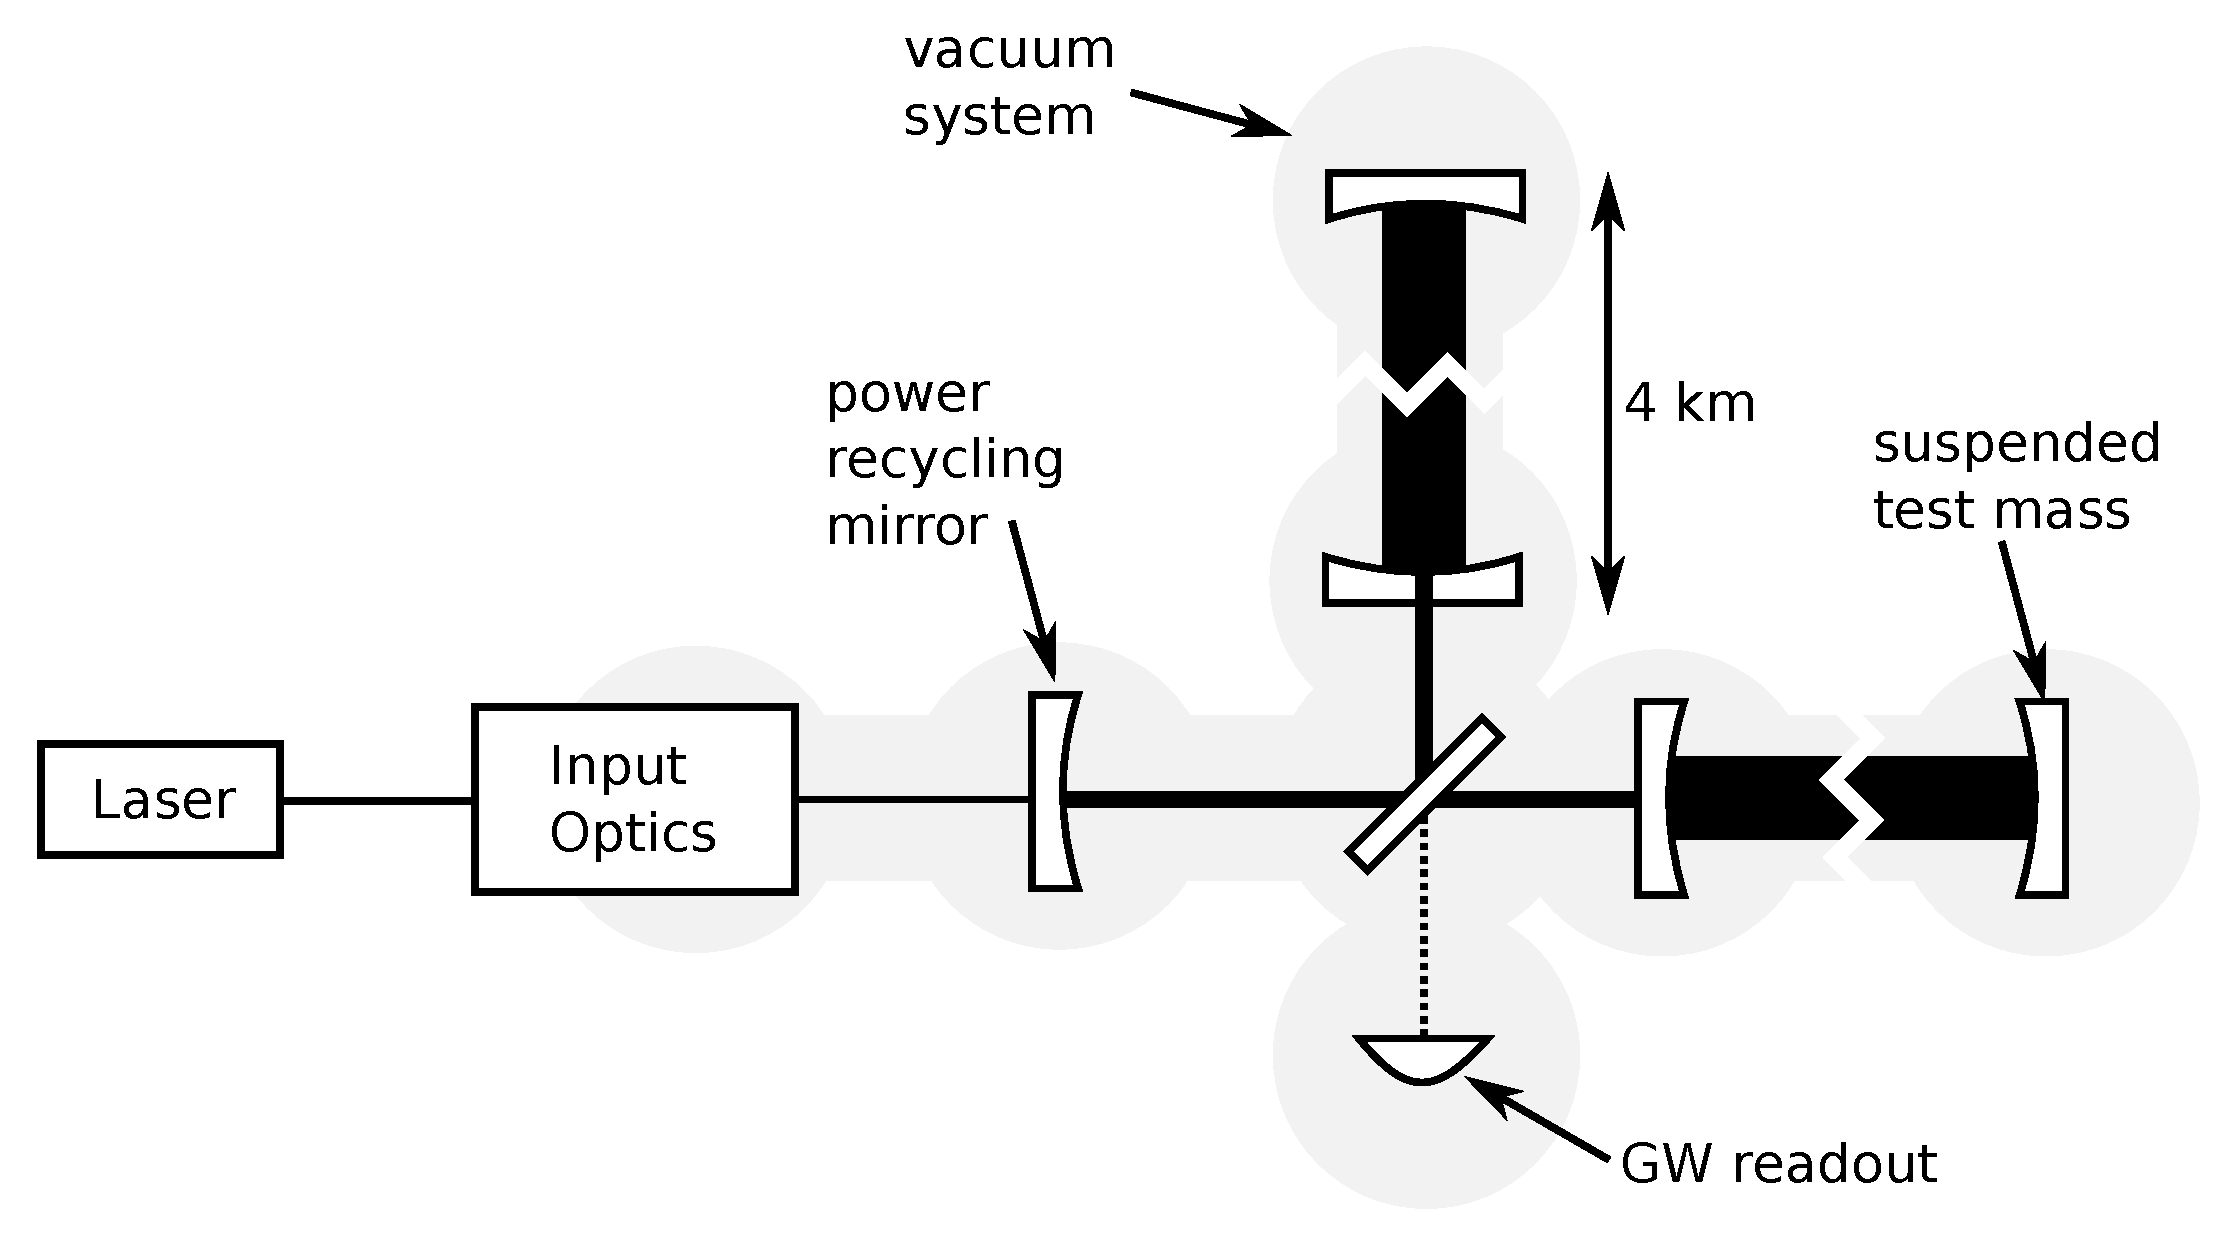
\includegraphics[width=0.8\textwidth]{figures/IFOschematic.pdf}
\caption{Power-recycled Fabry-Perot Michelson laser interferometer.}
\label{fig:IFOschematic}
\end{centering}
\end{figure}



\section{Measuring GW strain with light}
\subsection{Light as a photon} 
Consider two wave packets leaving the beam splitter of a Michelson
interferometer at the same time, each heading down a different arm. If
an appropriately polarized gravitational wave is present, the amount
of time the wave packet takes to travel down a stretched arm and back
is:
\begin{equation}
\label{eq:trt+} 
t_{rt+} = \frac{2 L}{c} \left( 1 + \frac{h_+}{2} \right)
\end{equation}
Likewise, for a compressed arm the roundtrip travel time is:
\begin{equation}
\label{eq:trt-} 
t_{rt-} = \frac{2 L}{c} \left( 1 - \frac{h_+}{2} \right)
\end{equation}
There is a non-zero $2Lh_+/c$ difference in arrival times at the beam splitter, a quantity
one could measure with an accurate stationary clock. This demonstrates intuitively that
a laser interferometer can detect gravitational waves.

It should be noted that we had to use the approximation that the
gravitational wave wavelength $\lambda_{gw}$ is much larger than the
interferometer arm length $L$. This means that the temporal variation
of $h_+(t)$ is negligible during the time it takes the photon to make
its roundtrip. Thus, $h_+$ is treated as a constant in
Eqs. \ref{eq:trt+} and \ref{eq:trt-}.


\subsection{Light as a wave}
The detector at the beam splitter is not a clock, but a photodetector
which is sensitive to phase. It would be informative, therefore, to express
the difference in arrival times as a difference in phase. To do so, we
must move away from the photon model and think about the wave model of
light.  The light wave's phase is given by $\phi = \omega t$ where $t$ is the proper time. Then, the
difference in phase between the two light beams after each has
completed its roundtrip is:
\begin{equation}
\Delta \phi = \phi_{rt+} - \phi_{rt-} = \frac{2 L \omega}{c} h_+
\end{equation}
Two time derivatives yields 
\begin{equation}
\frac{d^2\Delta \phi}{dt^2} = \frac{2 L \omega}{c} \partial_t \partial_t h_+.
\end{equation}
It can be shown \cite{Garfinkle2005Gauge} that the Riemann tensor in
the TT gauge is $R_{tkti}~=-\frac{1}{2}\partial_t \partial_t h_{ki}$,
and gauge invariant. Therefore, our
physically measurable quantity can be expressed as being manifestly
gauge invariant, proving that a laser interferometer can detect the
effect of gravitational waves.





\section{Power Recycled Michelson Interferometers}
\begin{itemize}
\item phase detection, sidebands
\item sub-systems, basic loops
\end{itemize}




\section{More Laser Power}




\section{Digital Control in LIGO}
The LIGO interferometers are interfaced through a digital control
system. 


